\section[MAGO]{Developing a \ac{MAGO}}

\begin{frame}{\insertsection}
    The result of a cooperation between:
        \begin{itemize}
            \item University of Zagreb Faculty of Organization and Informatics (\alert{UNIZG FOI}) and
            \item Universitat Politècnica de València (\alert{UPV}), Valencian Research Institute for Artificial Intelligence (\alert{VRAIN}).
        \end{itemize}

    \medskip
    The European Union and the Croatian Science Foundation fund this cooperation.
\end{frame}

\begin{frame}{\insertsection}
    \customFigure[1]{% how wide is the figure?
        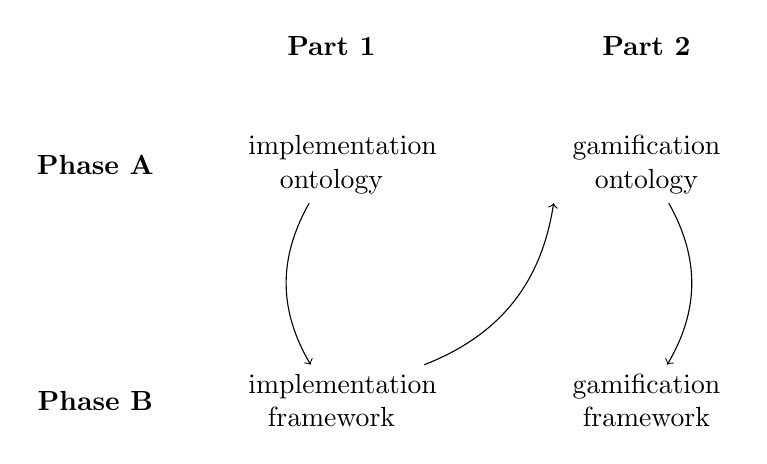
\begin{tikzpicture}
  \node [text width=6em, align=center] (4) at (0,3) {implementation ontology};
  \node [text width=6em, align=center] (1) at (0,0) {implementation framework};
  \node [text width=6em, align=center] (3) at (4,3) {gamification ontology};
  \node [text width=6em, align=center] (2) at (4,0) {gamification framework};
  
  \node (part 1) at (0,4.5) {\textbf{Part \RN{1}}};
  \node (part 2) at (4,4.5) {\textbf{Part \RN{2}}};
  \node (part 1) at (-3,3) {\textbf{Phase A}};
  \node (part 1) at (-3,0) {\textbf{Phase B}};
  
  \draw [->, bend right] (1.north east) to (3.south west);
  \draw [->, bend left] (3) to (2);
  \draw [->, bend right] (4) to (1);
\end{tikzpicture}

    }{The flow between the parts and the phases of this research}{fig: research-quick-overview-flow}
\end{frame}



\subsection{MAGO-Ag Ontology}

\begin{frame}{\insertsubsection}
    \begin{itemize}
        \item An ontology comprising concepts applicable to \alert{implementing \acp{MAS} as \acp{IVE}}.

        \item The \alert{main goal} of the ontology is to enable the modelling of a multiagent system in terms of implementation possibilities.

        \item The ontology contains a selection of modified and enriched concepts of the MAMbO5 ontology, a result of earlier cooperation \cite{okresaduric2019MAMbO5NewOntology}.

        \begin{itemize}
            \item e.g. Agent, Behaviour, Action, Process, Objective, Artefact
        \end{itemize}
    \end{itemize}
\end{frame}

\begin{frame}{\insertsubsection}
    \customFigure[1.3]{
        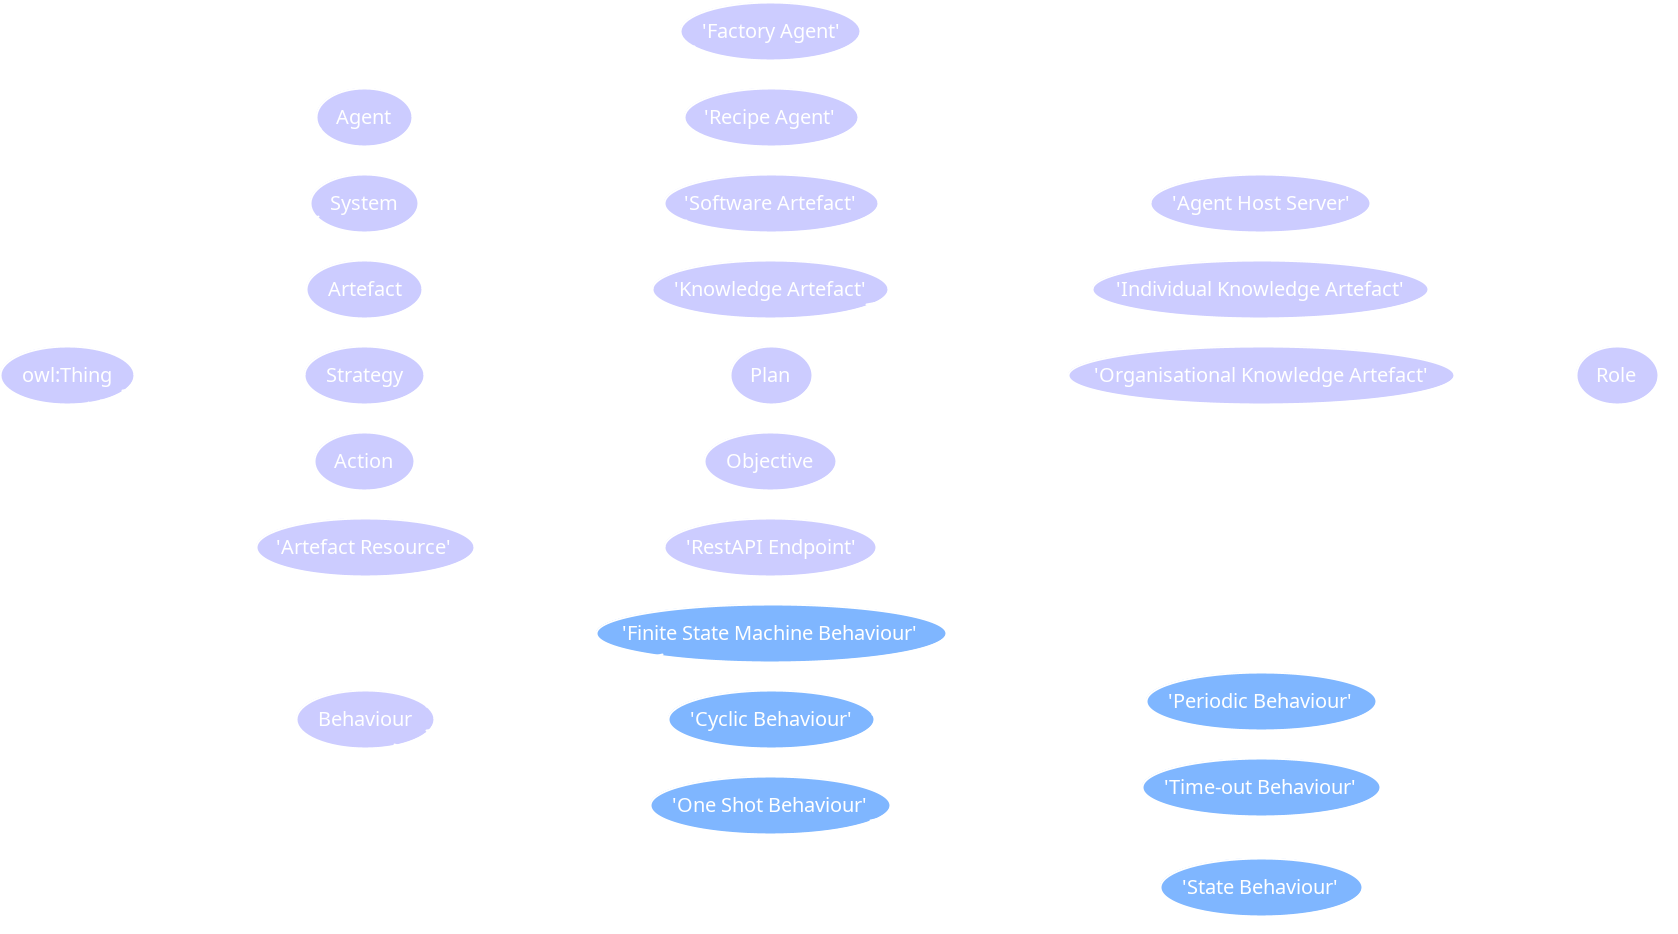
\includegraphics{Documents/241119 DSC Europe/Figures/onto dark.png}
    }{Visual relationship of the concepts of the MAGO-Ag ontology}{ontology concepts}
\end{frame}



\subsection{MAGO-Ag Framework}

\begin{frame}{\insertsubsection}
    \begin{itemize}
        \item The \alert{main objective} of the MAGO-Ag framework is to translate a \ac{MAS} modelled using the MAGO-Ag ontology into an \alert{implementation template} for a \ac{MAS} comprising SPADE agents.
    \end{itemize}
\end{frame}

\begin{frame}{\insertsubsection}
    \customFigure[0.6]{
        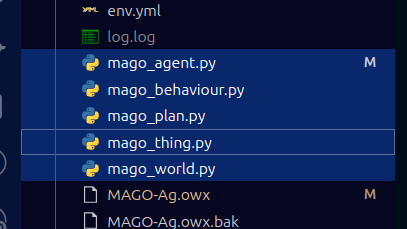
\includegraphics{Documents/241119 DSC Europe/Figures/Translation documents.png}
    }{Essential files of the translation process}{translation files}
\end{frame}

\activityFrame{\magoag framework}{}


\begin{frame}{\insertsubsection}
    \customFigure[0.6]{
        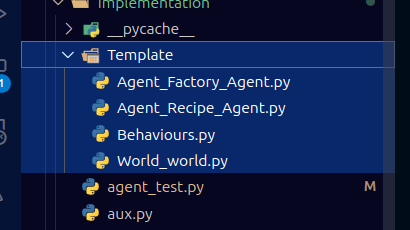
\includegraphics{Documents/241119 DSC Europe/Figures/Generated template files.png}
    }{Generated template files for the modelled system}{generated template files}
\end{frame}

\begin{frame}{\insertsubsection}
    \customFigure[1]{
        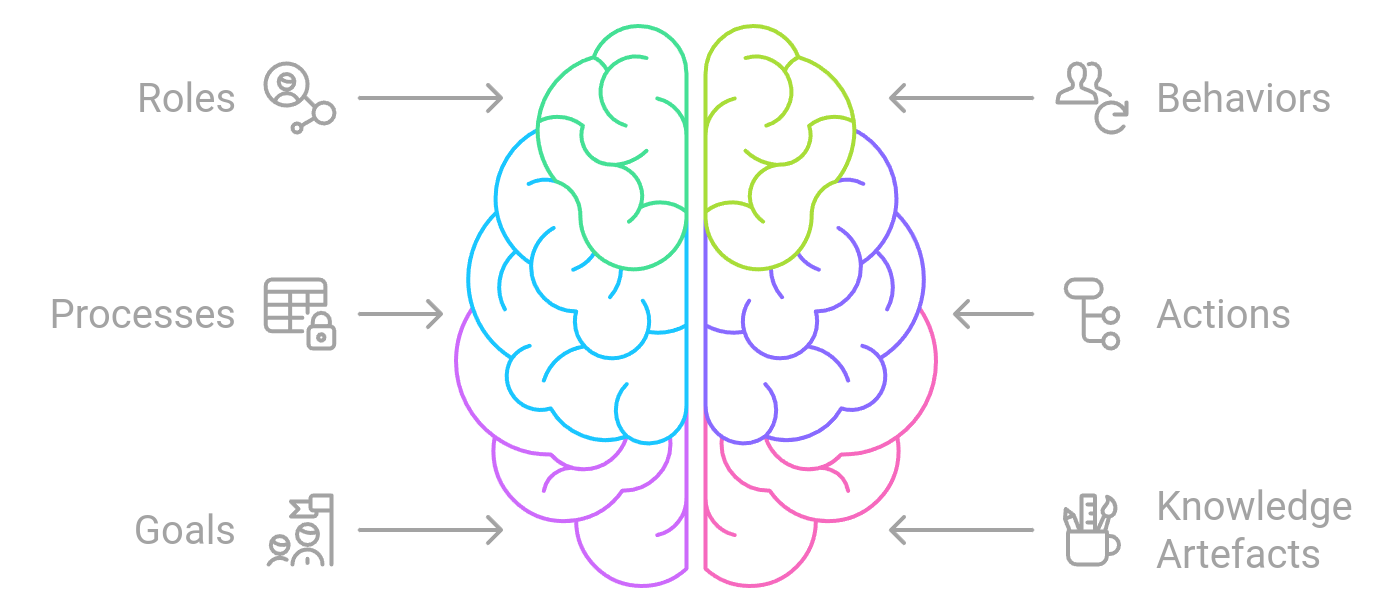
\includegraphics{Documents/241119 DSC Europe/Figures/Agent available knowledge dark.png}
    }{Pieces of knowledge available to agents after template generation}{available agent knowledge}
\end{frame}
